\documentclass{beamer}

\usepackage[utf8]{inputenc}
\usepackage[T1]{fontenc}
\usepackage{kantlipsum}
\usepackage{listings,xcolor}
\usepackage{inconsolata}
\usepackage{spverbatim}

\definecolor{dkgreen}{rgb}{0,.6,0}
\definecolor{dkblue}{rgb}{0,0,.6}
\definecolor{dkyellow}{cmyk}{0,0,.8,.3}

\lstset{
  language         = php,
  basicstyle       = \scriptsize\ttfamily,
  keywordstyle     = \color{dkblue},
  stringstyle      = \color{red},
  identifierstyle  = \color{dkgreen},
  commentstyle     = \color{gray},
  emph             =[1]{php},
  emphstyle        =[1]\color{black},
  emph             =[2]{if,and,or,else},
  emphstyle        =[2]\color{dkyellow}
  showstringspaces = false,
  numbers          = left,
  }

\usepackage{xstring}
\usepackage{catchfile}

\newcommand{\gitfolder}{.git}
\CatchFileDef{\headfull}{\gitfolder/HEAD}{}
\StrGobbleRight{\headfull}{1}[\head]
\StrBehind[2]{\head}{/}[\branch]
\CatchFileDef{\commit}{\gitfolder/refs/heads/\branch}{}
\StrGobbleRight{\commit}{1}[\longcommithash]

\newcommand{\gitrevisionlong}{%
	\longcommithash%
}

\newcommand{\gitrevisionsmall}{%
	\StrLeft{\longcommithash}{7}%
}


\title{Lazy collection}
\subtitle{Let your code procrastinate}
\institute{AFUP}
\date[2021]{Mai 2021}
\author[Pol]{Pol Dellaiera}
\logo{
    \vspace{-.3cm}
    \tikz{
        \node[opacity=0.15, inner sep=0.10cm, outer sep=0cm]{
            
\includegraphics[scale=0.35, keepaspectratio]{afup/style/logo/afup-icon+name-color}
        }
    }
}

\usetheme{afup}

% From https://jayrobwilliams.com/posts/2019/10/better-beamer
\makeatletter
\renewcommand{\itemize}[1][]{%
	\beamer@ifempty{#1}{}{\def\beamer@defaultospec{#1}}%
	\ifnum \@itemdepth >2\relax\@toodeep\else
	\advance\@itemdepth\@ne
	\beamer@computepref\@itemdepth% sets \beameritemnestingprefix
	\usebeamerfont{itemize/enumerate \beameritemnestingprefix body}%
	\usebeamercolor[fg]{itemize/enumerate \beameritemnestingprefix body}%
	\usebeamertemplate{itemize/enumerate \beameritemnestingprefix body begin}%
	\list
	{\usebeamertemplate{itemize \beameritemnestingprefix item}}
	{\def\makelabel##1{%
			{%
				\hss\llap{{%
						\usebeamerfont*{itemize \beameritemnestingprefix item}%
						\usebeamercolor[fg]{itemize \beameritemnestingprefix item}##1}}%
			}%
		}%
	}
	\fi%
	\setlength\itemsep{\fill}
	\ifnum \@itemdepth >1
	\vfill
	\fi%
	\beamer@cramped%
	\raggedright%
	\beamer@firstlineitemizeunskip%
}
\def\enditemize{\ifhmode\unskip\fi\endlist%
	\usebeamertemplate{itemize/enumerate \beameritemnestingprefix body end}
	\ifnum \@itemdepth >1
	\vfil
	\fi%
}
\makeatother

\usepackage{environ}

\newcommand{\sepframe}[2]{
    \setbeamercolor{background canvas}{bg=afupbluebackground}

    \begin{frame}[noframenumbering,plain]
        \begin{tikzpicture}[remember picture,overlay]
            \fill[afuppink] (0,0) rectangle(.05,\paperheight);
        \end{tikzpicture}
      \begin{tikzpicture}[remember picture,overlay]
          \ifx\insertframesubtitle\@empty%
              {\node[anchor=west, afupblue, font=\huge] at (0,.25){\uppercase\expandafter{#1}};}
          \else%
              {
                  \node[anchor= west, afupblue, font=\huge] at (0,.25){\uppercase\expandafter{#1}};%
                  \node[anchor= west, afuppink,font=\small] at (0,-.5){\uppercase\expandafter{#2}};}%
          \fi
      \end{tikzpicture}

      \begin{tikzpicture}[remember picture, overlay]
          \node at (current page.south east) {
              
\includegraphics[trim=0 -4cm -4cm 0, scale=.35, keepaspectratio]{src/afup/style/logo/afup-icon-color}
            };
      \end{tikzpicture}
    \end{frame}
  }

\NewEnviron{sepFrameA}[3][]{%
    \begin{frame}
        \begin{columns}
            \column{\paperwidth}
                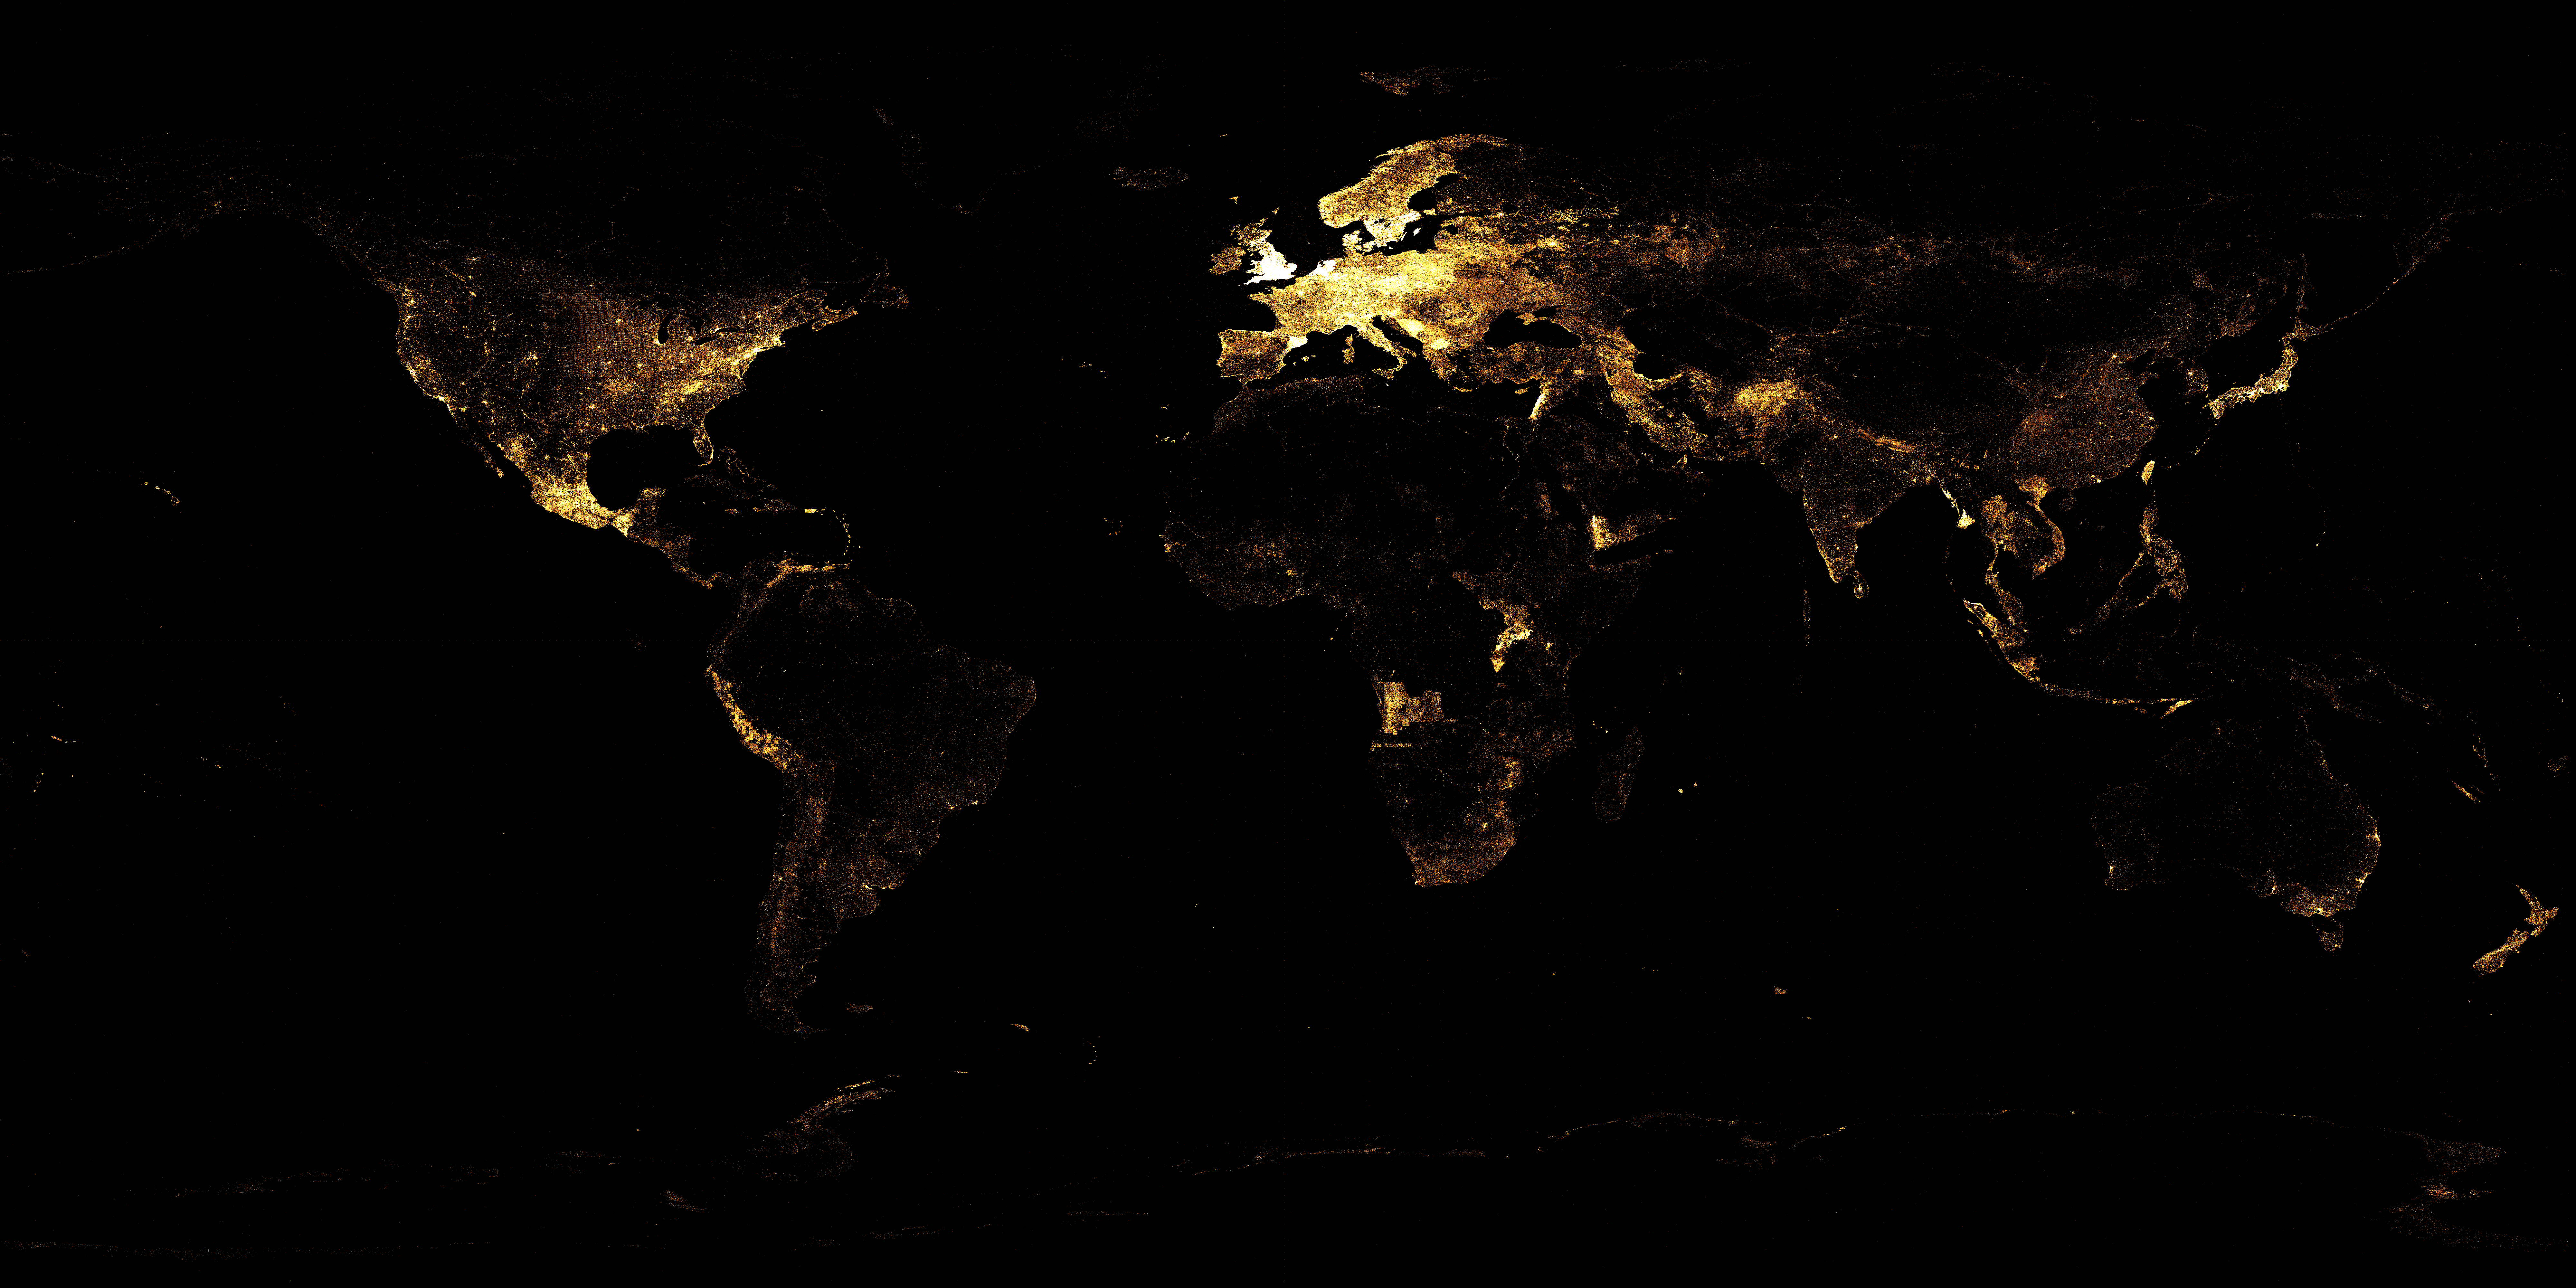
\includegraphics[width=\the\paperwidth, height=.5\paperheight]{src/afup/style/logo/bg1}
            \begin{tikzpicture}
                \node[shape=rectangle, text opacity=1,minimum height=.5\paperheight, minimum width=\paperwidth, anchor=south]{
                    \BODY
                };
            \end{tikzpicture}
          \end{columns}
    \end{frame}
}

\NewEnviron{sepFrameB}[3][]{%
    \begin{frame}
        \begin{columns}
            \column{.5\paperwidth}
                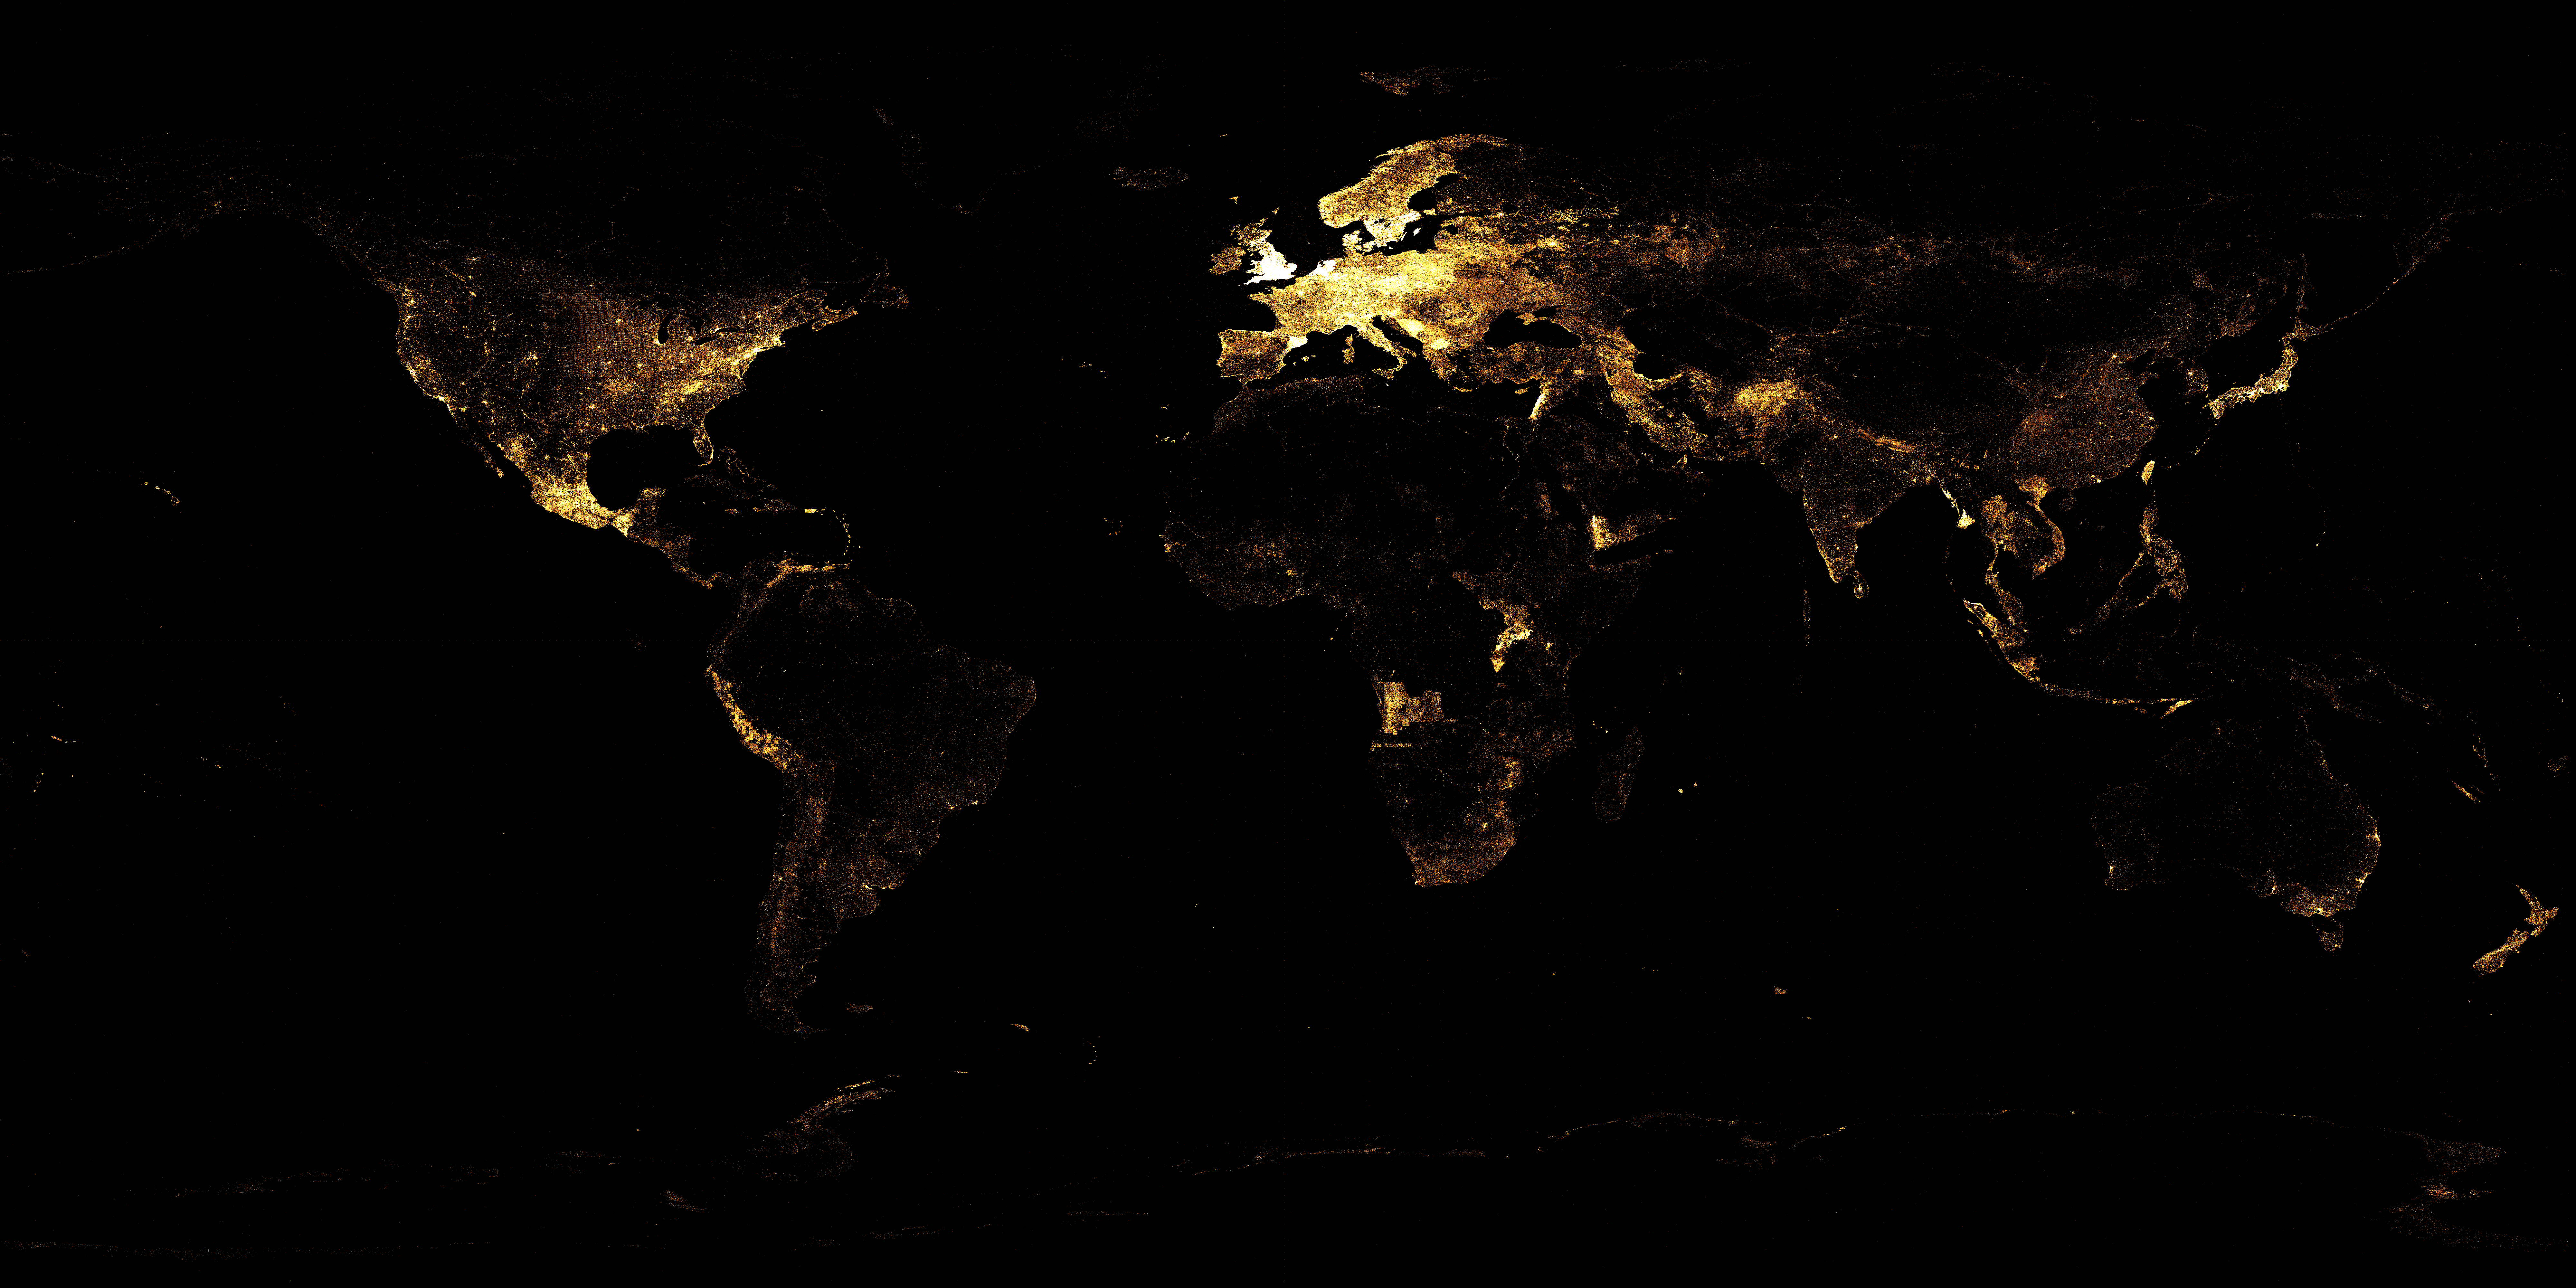
\includegraphics[width=.5\paperwidth, height=\paperheight]{src/afup/style/logo/bg1}
            \column{.5\paperwidth}
                \begin{tikzpicture}
                    \node[shape=rectangle, text opacity=1,minimum height=\paperheight, minimum width=.5\paperwidth, anchor=east]{
                        \BODY
                    };
                \end{tikzpicture}
        \end{columns}
    \end{frame}
}


% To read: https://tex.stackexchange.com/questions/113410/removing-sidebar-from-a-single-beamer-frame
% To read: https://github.com/deuslirio/UFGTeX-Presentation
% To read: https://github.com/matze/mtheme


\begin{document}

\begin{frame}[plain]
	\titlepage{}
\end{frame}

\begin{frameA}{Frame A title}{Frame A subtitle}
\end{frameA}

\begin{frameB}{Frame B title}{Frame B subtitle}
\end{frameB}

\begin{frameC}{Frame C title}{Frame C subtitle}
\end{frameC}

\begin{frameD}{Frame D title}{Frame D subtitle}
\end{frameD}

\section{section 1}
\begin{frame}{Une collection}{Une définition simple}
    \begin{itemize}
        \item Une collection est une structure unifiée pour représenter et manipuler un ensemble de données.
        \item Permettant de les manipuler indépendamment de ce qu'elles contiennent.
        \item Elle permettent de réduire l'effort tout en améliorant les performances\footnotemark.
        \item Favorise l'interoperabilité
        \item Favorise la réutilisation
        \item Inclus des implémentations et algorithmes pour manipuler les données
    \end{itemize}

    \footnotetext[1]{A test footnote in the first column}
\end{frame}

\begin{frame}{Pourquoi}{Fixer les incohérences}
    PHP dispose de plusieurs structures natives propice à l'itération

    \begin{itemize}[<+->]
        \item \texttt{array}
        \item Interface \texttt{ArrayAccess}
        \item Iterateur
        \item Generateur
    \end{itemize}
\end{frame}

\begin{frame}{Pourquoi}{Fixer les incohérences}
    PHP dispose de plusieurs fonctions natives propice à l'itération

    \begin{itemize}[<+->]
        \item \texttt{array\_map()}
        \item \texttt{array\_filter()}
        \item \texttt{array\_reduce()}
        \item \texttt{iterator\_to\_array()}
    \end{itemize}
\end{frame}

\begin{frame}{Pourquoi}{Fixer les incohérences}
    PHP dispose de plusieurs structure indispensable pour itérer

    \begin{itemize}[<+->]
        \item \texttt{for}
        \item \texttt{foreach}
        \item \texttt{while}
    \end{itemize}
\end{frame}

\begin{frame}{Incohérences}{array}
    \begin{itemize}[<+->]
        \item Manque de consistence (\texttt{array\_*()})
        \item Pas de vérification des types
        \item Performances
        \item Pas de gestion des erreurs
    \end{itemize}
\end{frame}

\begin{frame}{Incohérences}{php}
    \begin{itemize}[<+->]
        \item Manque de consistence dans les fonctions du genre \texttt{array\_*()}
        \item Les fonctions d'itérations ne fonctionnent que pour les arrays. Quid du type \texttt{iterable}?
    \end{itemize}
\end{frame}

\begin{frame}{Incohérences}{php}
    \begin{itemize}[<+->]
        \item \texttt{array\_map(\$callable, \$array)}
        \item \texttt{array\_map(\$array, \$callable)}
    \end{itemize}
\end{frame}

\begin{frame}
	\frametitle{Incohérences}
    \framesubtitle{PHP/array\_map()}

    Un array est composé de\ldots

    \begin{itemize}[<+->]
        \item clés
        \item valeurs
    \end{itemize}

    \pause

    Cependant\ldots

    \pause

    \begin{itemize}[<+->]
        \item Signature: \texttt{array\_map(\$callable, \$array)}
        \item Callable: \texttt{\$callable(\$value)}
    \end{itemize}
\end{frame}

\begin{frame}{Incohérences}{Pourquoi?}
    \begin{itemize}[<+->]
        \item Pourquoi un tableau est composé de 2 types de données?
        \item Pourquoi la plupart des fonctions natives ne nous permettent pas d'utiliser les 2?
    \end{itemize}
\end{frame}

\begin{frameC}{Bref\ldots}\end{frameC}

\begin{frame}{Collections}{ça existe déjà!}
    \begin{itemize}[<+->]
        \item doctrine/collection
        \item voku/Arrayy
        \item Laravel
        \item CakePHP
    \end{itemize}
\end{frame}

\begin{frame}{Collections}{Pourquoi?}
    \begin{itemize}[<+->]
        \item Unifier la manière de travailler avec des ensemble de données?
        \item Optimiser les algorithmes?
        \item faciliter l'emploi de certaines fonctionnalités?
    \end{itemize}
\end{frame}

\begin{frame}{Collections}{Problèmes rencontrés?}
    \begin{itemize}[<+->]
        \item La plupart sont des wrapper de fonctions natives PHP
        \item La plupart se basent sur des array
    \end{itemize}
\end{frame}

\begin{frame}[fragile]
    \begin{lstlisting}[firstnumber=1]
        <?php

        $array = // huge dataset
    \end{lstlisting}
\end{frame}

\begin{frame}[fragile]
    \begin{lstlisting}[firstnumber=1]
        <?php

        $size = 1000;

        $array = range(0, $size ** 3);
    \end{lstlisting}
\end{frame}

\begin{frame}[fragile]
    \begin{spverbatim}
        PHP Fatal error: Allowed memory size of 536870912 bytes exhausted (tried to allocate 34359738376 bytes) in example.php on line 5
    \end{spverbatim}
\end{frame}

\begin{frame}{Thunk}{Définition}
    \begin{quote}
        A thunk is a value that is yet to be evaluated. It is used in Haskell systems that implement non-strict semantics by lazy evaluation.

        \pause

        A thunk is a function that wraps an expression to delay its evaluation.

        \pause

        The term originated as a humorous past-tense version of "think".
    \end{quote}
\end{frame}

\begin{frame}[fragile]{Thunk}{Example}
    \begin{lstlisting}
    <?php

    // Calculation of 1 + 2 is immediate
    // $x === 3
    $x = 1 + 2;
    \end{lstlisting}

    \pause

    \begin{lstlisting}[firstnumber=6]
    // Calculation of 1 + 2 is delayed
    // $foo can be called later to perform the calculation
    // $foo is a thunk!
    $foo = fn () => 1 + 2;
    \end{lstlisting}
\end{frame}

\begin{frame}
    \begin{quote}
        Je fais du vélo le matin, je voudrais ne pas respirer la poussière générée
        par ces datacenters fous fonctionnant si mal avec des algorithmes,
        car on se donne entre les mains un pouvoir qu'il ne maîtrise pas.

        \begin{flushright}
            \tiny{---Julien Pauli}
        \end{flushright}
    \end{quote}
\end{frame}

\begin{frame}
    \begin{quote}
        Si vous voulez être un meilleur programmeur, apprenez un autre language que
        le PHP. Si possible un language fonctionnel.

        \begin{flushright}
            \tiny{---Larry Garfield}
        \end{flushright}
    \end{quote}
\end{frame}

\begin{frame}{Schematisons}{une évaluation traditionnelle}
    \begin{center}
        \texttt{
            \begin{tabular}{|l|l|l|}
                \hline
                0 & 1 & 2 \\ \hline
                a & b & a \\ \hline
            \end{tabular}
        }

        \pause

        $\xrightarrow{\texttt{flip()}}$

        \pause

        \texttt{
            \begin{tabular}{|l|l|l|}
                \hline
                a & b \\ \hline
                2 & 1 \\ \hline
            \end{tabular}
        }

        \pause

        $\xrightarrow{\texttt{flip()}}$

        \pause

        \texttt{
            \begin{tabular}{|l|l|l|}
                \hline
                2 & 1 \\ \hline
                a & b \\ \hline
            \end{tabular}
        }
    \end{center}
\end{frame}

\begin{frame}{Schematisons}{evaluation \textit{lazy}}
    \newcolumntype{t}{>{\tt}c}
    \begin{center}
        \[
            \left[ \begin{array}{tt}
                0 \Rightarrow a \\
                1 \Rightarrow b \\
                2 \Rightarrow a
            \end{array} \right]
            \pause
            \xrightarrow{\texttt{array\_flip()}}
            \left[ \begin{array}{tt}
                \only<2->{a \Rightarrow 0} \\
                \only<4->{b \Rightarrow 1} \\
                \only<6->{a \Rightarrow 2}
            \end{array} \right]
            \pause
            \xrightarrow{\texttt{array\_flip()}}
            \left[ \begin{array}{tt}
                \only<3->{0 \Rightarrow a} \\
                \only<5->{1 \Rightarrow b} \\
                \only<7->{2 \Rightarrow a}
            \end{array} \right]
        \]
    \end{center}
\end{frame}

\begin{frame}{Schematisons}{evaluation \textit{lazy}}
    \newcolumntype{t}{>{\tt}c}
    \begin{center}
        \begin{minipage}[adjusting]{.65\textwidth}
            \begin{math}
                \left[ \begin{array}{tt}
                    0 \Rightarrow \left[ \begin{array}{tt} a \Rightarrow A\end{array} \right] \\
                    1 \Rightarrow \left[ \begin{array}{tt} b \Rightarrow B\end{array} \right] \\
                    2 \Rightarrow \left[ \begin{array}{tt} c \Rightarrow C\end{array} \right]
                \end{array} \right]
                \pause
                \xrightarrow{\texttt{array\_flip()}}\newline
                \left[ \begin{array}{tt}
                    \only<2->{\left[ \begin{array}{tt} a \Rightarrow A\end{array} \right] \Rightarrow 0} \\
                    \only<4->{\left[ \begin{array}{tt} b \Rightarrow B\end{array} \right] \Rightarrow 1} \\
                    \only<6->{\left[ \begin{array}{tt} c \Rightarrow C\end{array} \right] \Rightarrow 2}
                \end{array} \right]
                \pause
                \xrightarrow{\texttt{array\_flip()}}\newline
                \left[ \begin{array}{tt}
                    \only<3->{0 \Rightarrow \left[ \begin{array}{tt} a \Rightarrow A\end{array} \right]} \\
                    \only<5->{1 \Rightarrow \left[ \begin{array}{tt} b \Rightarrow B\end{array} \right]} \\
                    \only<7->{2 \Rightarrow \left[ \begin{array}{tt} c \Rightarrow C\end{array} \right]}
                \end{array} \right]
            \end{math}
        \end{minipage}
    \end{center}
\end{frame}


\end{document}
